
%% bare_conf.tex
%% V1.3
%% 2007/01/11
%% by Michael Shell
%% See:
%% http://www.michaelshell.org/
%% for current contact information.
%%
%% This is a skeleton file demonstrating the use of IEEEtran.cls
%% (requires IEEEtran.cls version 1.7 or later) with an IEEE conference paper.
%%
%% Support sites:
%% http://www.michaelshell.org/tex/ieeetran/
%% http://www.ctan.org/tex-archive/macros/latex/contrib/IEEEtran/
%% and
%% http://www.ieee.org/

%%*************************************************************************
%% Legal Notice:
%% This code is offered as-is without any warranty either expressed or
%% implied; without even the implied warranty of MERCHANTABILITY or
%% FITNESS FOR A PARTICULAR PURPOSE! 
%% User assumes all risk.
%% In no event shall IEEE or any contributor to this code be liable for
%% any damages or losses, including, but not limited to, incidental,
%% consequential, or any other damages, resulting from the use or misuse
%% of any information contained here.
%%
%% All comments are the opinions of their respective authors and are not
%% necessarily endorsed by the IEEE.
%%
%% This work is distributed under the LaTeX Project Public License (LPPL)
%% ( http://www.latex-project.org/ ) version 1.3, and may be freely used,
%% distributed and modified. A copy of the LPPL, version 1.3, is included
%% in the base LaTeX documentation of all distributions of LaTeX released
%% 2003/12/01 or later.
%% Retain all contribution notices and credits.
%% ** Modified files should be clearly indicated as such, including  **
%% ** renaming them and changing author support contact information. **
%%
%% File list of work: IEEEtran.cls, IEEEtran_HOWTO.pdf, bare_adv.tex,
%%                    bare_conf.tex, bare_jrnl.tex, bare_jrnl_compsoc.tex
%%*************************************************************************

% *** Authors should verify (and, if needed, correct) their LaTeX system  ***
% *** with the testflow diagnostic prior to trusting their LaTeX platform ***
% *** with production work. IEEE's font choices can trigger bugs that do  ***
% *** not appear when using other class files.                            ***
% The testflow support page is at:
% http://www.michaelshell.org/tex/testflow/



% Note that the a4paper option is mainly intended so that authors in
% countries using A4 can easily print to A4 and see how their papers will
% look in print - the typesetting of the document will not typically be
% affected with changes in paper size (but the bottom and side margins will).
% Use the testflow package mentioned above to verify correct handling of
% both paper sizes by the user's LaTeX system.
%
% Also note that the "draftcls" or "draftclsnofoot", not "draft", option
% should be used if it is desired that the figures are to be displayed in
% draft mode.
%
\documentclass[conference, compsoc]{IEEEtran}
% Add the compsoc option for Computer Society conferences.
%
% If IEEEtran.cls has not been installed into the LaTeX system files,
% manually specify the path to it like:
% \documentclass[conference]{../sty/IEEEtran}





% Some very useful LaTeX packages include:
% (uncomment the ones you want to load)


% *** MISC UTILITY PACKAGES ***
%
%\usepackage{ifpdf}
% Heiko Oberdiek's ifpdf.sty is very useful if you need conditional
% compilation based on whether the output is pdf or dvi.
% usage:
% \ifpdf
%   % pdf code
% \else
%   % dvi code
% \fi
% The latest version of ifpdf.sty can be obtained from:
% http://www.ctan.org/tex-archive/macros/latex/contrib/oberdiek/
% Also, note that IEEEtran.cls V1.7 and later provides a builtin
% \ifCLASSINFOpdf conditional that works the same way.
% When switching from latex to pdflatex and vice-versa, the compiler may
% have to be run twice to clear warning/error messages.






% *** CITATION PACKAGES ***
%
%\usepackage{cite}
% cite.sty was written by Donald Arseneau
% V1.6 and later of IEEEtran pre-defines the format of the cite.sty package
% \cite{} output to follow that of IEEE. Loading the cite package will
% result in citation numbers being automatically sorted and properly
% "compressed/ranged". e.g., [1], [9], [2], [7], [5], [6] without using
% cite.sty will become [1], [2], [5]--[7], [9] using cite.sty. cite.sty's
% \cite will automatically add leading space, if needed. Use cite.sty's
% noadjust option (cite.sty V3.8 and later) if you want to turn this off.
% cite.sty is already installed on most LaTeX systems. Be sure and use
% version 4.0 (2003-05-27) and later if using hyperref.sty. cite.sty does
% not currently provide for hyperlinked citations.
% The latest version can be obtained at:
% http://www.ctan.org/tex-archive/macros/latex/contrib/cite/
% The documentation is contained in the cite.sty file itself.






% *** GRAPHICS RELATED PACKAGES ***
%
  %\ifCLASSINFOpdf
   \usepackage[pdftex]{graphicx}
  % declare the path(s) where your graphic files are
  % \graphicspath{{../pdf/}{../jpeg/}}
  % and their extensions so you won't have to specify these with
  % every instance of \includegraphics
  % \DeclareGraphicsExtensions{.pdf,.jpeg,.png}
\else
  % or other class option (dvipsone, dvipdf, if not using dvips). graphicx
  % will default to the driver specified in the system graphics.cfg if no
  % driver is specified.
  % \usepackage[dvips]{graphicx}
  % declare the path(s) where your graphic files are
  % \graphicspath{{../eps/}}
  % and their extensions so you won't have to specify these with
  % every instance of \includegraphics
  % \DeclareGraphicsExtensions{.eps}
\fi
% graphicx was written by David Carlisle and Sebastian Rahtz. It is
% required if you want graphics, photos, etc. graphicx.sty is already
% installed on most LaTeX systems. The latest version and documentation can
% be obtained at: 
% http://www.ctan.org/tex-archive/macros/latex/required/graphics/
% Another good source of documentation is "Using Imported Graphics in
% LaTeX2e" by Keith Reckdahl which can be found as epslatex.ps or
% epslatex.pdf at: http://www.ctan.org/tex-archive/info/
%
% latex, and pdflatex in dvi mode, support graphics in encapsulated
% postscript (.eps) format. pdflatex in pdf mode supports graphics
% in .pdf, .jpeg, .png and .mps (metapost) formats. Users should ensure
% that all non-photo figures use a vector format (.eps, .pdf, .mps) and
% not a bitmapped formats (.jpeg, .png). IEEE frowns on bitmapped formats
% which can result in "jaggedy"/blurry rendering of lines and letters as
% well as large increases in file sizes.
%
% You can find documentation about the pdfTeX application at:
% http://www.tug.org/applications/pdftex





% *** MATH PACKAGES ***
%
%\usepackage[cmex10]{amsmath}
% A popular package from the American Mathematical Society that provides
% many useful and powerful commands for dealing with mathematics. If using
% it, be sure to load this package with the cmex10 option to ensure that
% only type 1 fonts will utilized at all point sizes. Without this option,
% it is possible that some math symbols, particularly those within
% footnotes, will be rendered in bitmap form which will result in a
% document that can not be IEEE Xplore compliant!
%
% Also, note that the amsmath package sets \interdisplaylinepenalty to 10000
% thus preventing page breaks from occurring within multiline equations. Use:
%\interdisplaylinepenalty=2500
% after loading amsmath to restore such page breaks as IEEEtran.cls normally
% does. amsmath.sty is already installed on most LaTeX systems. The latest
% version and documentation can be obtained at:
% http://www.ctan.org/tex-archive/macros/latex/required/amslatex/math/





% *** SPECIALIZED LIST PACKAGES ***
%
%\usepackage{algorithmic}
% algorithmic.sty was written by Peter Williams and Rogerio Brito.
% This package provides an algorithmic environment fo describing algorithms.
% You can use the algorithmic environment in-text or within a figure
% environment to provide for a floating algorithm. Do NOT use the algorithm
% floating environment provided by algorithm.sty (by the same authors) or
% algorithm2e.sty (by Christophe Fiorio) as IEEE does not use dedicated
% algorithm float types and packages that provide these will not provide
% correct IEEE style captions. The latest version and documentation of
% algorithmic.sty can be obtained at:
% http://www.ctan.org/tex-archive/macros/latex/contrib/algorithms/
% There is also a support site at:
% http://algorithms.berlios.de/index.html
% Also of interest may be the (relatively newer and more customizable)
% algorithmicx.sty package by Szasz Janos:
% http://www.ctan.org/tex-archive/macros/latex/contrib/algorithmicx/




% *** ALIGNMENT PACKAGES ***
%
%\usepackage{array}
% Frank Mittelbach's and David Carlisle's array.sty patches and improves
% the standard LaTeX2e array and tabular environments to provide better
% appearance and additional user controls. As the default LaTeX2e table
% generation code is lacking to the point of almost being broken with
% respect to the quality of the end results, all users are strongly
% advised to use an enhanced (at the very least that provided by array.sty)
% set of table tools. array.sty is already installed on most systems. The
% latest version and documentation can be obtained at:
% http://www.ctan.org/tex-archive/macros/latex/required/tools/


%\usepackage{mdwmath}
%\usepackage{mdwtab}
% Also highly recommended is Mark Wooding's extremely powerful MDW tools,
% especially mdwmath.sty and mdwtab.sty which are used to format equations
% and tables, respectively. The MDWtools set is already installed on most
% LaTeX systems. The lastest version and documentation is available at:
% http://www.ctan.org/tex-archive/macros/latex/contrib/mdwtools/


% IEEEtran contains the IEEEeqnarray family of commands that can be used to
% generate multiline equations as well as matrices, tables, etc., of high
% quality.


%\usepackage{eqparbox}
% Also of notable interest is Scott Pakin's eqparbox package for creating
% (automatically sized) equal width boxes - aka "natural width parboxes".
% Available at:
% http://www.ctan.org/tex-archive/macros/latex/contrib/eqparbox/





% *** SUBFIGURE PACKAGES ***
%\usepackage[tight,footnotesize]{subfigure}
% subfigure.sty was written by Steven Douglas Cochran. This package makes it
% easy to put subfigures in your figures. e.g., "Figure 1a and 1b". For IEEE
% work, it is a good idea to load it with the tight package option to reduce
% the amount of white space around the subfigures. subfigure.sty is already
% installed on most LaTeX systems. The latest version and documentation can
% be obtained at:
% http://www.ctan.org/tex-archive/obsolete/macros/latex/contrib/subfigure/
% subfigure.sty has been superceeded by subfig.sty.



%\usepackage[caption=false]{caption}
%\usepackage[font=footnotesize]{subfig}
% subfig.sty, also written by Steven Douglas Cochran, is the modern
% replacement for subfigure.sty. However, subfig.sty requires and
% automatically loads Axel Sommerfeldt's caption.sty which will override
% IEEEtran.cls handling of captions and this will result in nonIEEE style
% figure/table captions. To prevent this problem, be sure and preload
% caption.sty with its "caption=false" package option. This is will preserve
% IEEEtran.cls handing of captions. Version 1.3 (2005/06/28) and later 
% (recommended due to many improvements over 1.2) of subfig.sty supports
% the caption=false option directly:
%\usepackage[caption=false,font=footnotesize]{subfig}
%
% The latest version and documentation can be obtained at:
% http://www.ctan.org/tex-archive/macros/latex/contrib/subfig/
% The latest version and documentation of caption.sty can be obtained at:
% http://www.ctan.org/tex-archive/macros/latex/contrib/caption/




% *** FLOAT PACKAGES ***
%
%\usepackage{fixltx2e}
% fixltx2e, the successor to the earlier fix2col.sty, was written by
% Frank Mittelbach and David Carlisle. This package corrects a few problems
% in the LaTeX2e kernel, the most notable of which is that in current
% LaTeX2e releases, the ordering of single and double column floats is not
% guaranteed to be preserved. Thus, an unpatched LaTeX2e can allow a
% single column figure to be placed prior to an earlier double column
% figure. The latest version and documentation can be found at:
% http://www.ctan.org/tex-archive/macros/latex/base/



%\usepackage{stfloats}
% stfloats.sty was written by Sigitas Tolusis. This package gives LaTeX2e
% the ability to do double column floats at the bottom of the page as well
% as the top. (e.g., "\begin{figure*}[!b]" is not normally possible in
% LaTeX2e). It also provides a command:
%\fnbelowfloat
% to enable the placement of footnotes below bottom floats (the standard
% LaTeX2e kernel puts them above bottom floats). This is an invasive package
% which rewrites many portions of the LaTeX2e float routines. It may not work
% with other packages that modify the LaTeX2e float routines. The latest
% version and documentation can be obtained at:
% http://www.ctan.org/tex-archive/macros/latex/contrib/sttools/
% Documentation is contained in the stfloats.sty comments as well as in the
% presfull.pdf file. Do not use the stfloats baselinefloat ability as IEEE
% does not allow \baselineskip to stretch. Authors submitting work to the
% IEEE should note that IEEE rarely uses double column equations and
% that authors should try to avoid such use. Do not be tempted to use the
% cuted.sty or midfloat.sty packages (also by Sigitas Tolusis) as IEEE does
% not format its papers in such ways.





% *** PDF, URL AND HYPERLINK PACKAGES ***
%
%\usepackage{url}
% url.sty was written by Donald Arseneau. It provides better support for
% handling and breaking URLs. url.sty is already installed on most LaTeX
% systems. The latest version can be obtained at:
% http://www.ctan.org/tex-archive/macros/latex/contrib/misc/
% Read the url.sty source comments for usage information. Basically,
% \url{my_url_here}.





% *** Do not adjust lengths that control margins, column widths, etc. ***
% *** Do not use packages that alter fonts (such as pslatex).         ***
% There should be no need to do such things with IEEEtran.cls V1.6 and later.
% (Unless specifically asked to do so by the journal or conference you plan
% to submit to, of course. )


% correct bad hyphenation here
\hyphenation{op-tical net-works semi-conduc-tor}


\begin{document}
%
% paper title
% can use linebreaks \\ within to get better formatting as desired
\title{Cloud Computing and Web based-application in IT environment}


% author names and affiliations
% use a multiple column layout for up to two different
% affiliations

\author{\IEEEauthorblockN{Mohammed Altemimi (P47901)}
\IEEEauthorblockA{dept. FTSM\\
Mohammed Alaa Hussein Altemimi\\
UKM University , Malaysia \\
goodprogrammer2005@yahoo.com}
\and
\IEEEauthorblockN{}
\IEEEauthorblockA{\\ }}

% conference papers do not typically use \thanks and this command
% is locked out in conference mode. If really needed, such as for
% the acknowledgment of grants, issue a \IEEEoverridecommandlockouts
% after \documentclass

% for over three affiliations, or if they all won't fit within the width
% of the page, use this alternative format:
% 
%\author{\IEEEauthorblockN{Michael Shell\IEEEauthorrefmark{1},
%Homer Simpson\IEEEauthorrefmark{2},
%James Kirk\IEEEauthorrefmark{3}, 
%Montgomery Scott\IEEEauthorrefmark{3} and
%Eldon Tyrell\IEEEauthorrefmark{4}}
%\IEEEauthorblockA{\IEEEauthorrefmark{1}School of Electrical and Computer Engineering\\
%Georgia Institute of Technology,
%Atlanta, Georgia 30332--0250\\ Email: see http://www.michaelshell.org/contact.html}
%\IEEEauthorblockA{\IEEEauthorrefmark{2}Twentieth Century Fox, Springfield, USA\\
%Email: homer@thesimpsons.com}
%\IEEEauthorblockA{\IEEEauthorrefmark{3}Starfleet Academy, San Francisco, California 96678-2391\\
%Telephone: (800) 555--1212, Fax: (888) 555--1212}
%\IEEEauthorblockA{\IEEEauthorrefmark{4}Tyrell Inc., 123 Replicant Street, Los Angeles, California 90210--4321}}




% use for special paper notices
%\IEEEspecialpapernotice{(Invited Paper)}




% make the title area
\maketitle


\begin{abstract}
%\boldmath
In this paper we describe on the study of cloud computing in current IT environment involve defines Cloud computing as well as the web based-application. In this paper also, presents some representative Cloud platforms especially those developed in industries, it will try to elaborate on the issue of how cloud computing will change the current business and what will be happen in the future as well as and concludes with the need for convergence of competing IT. Today your business needs to respond
in Internet time with new services, capabilities, and offerings to stay ahead of its competitors. 

\end{abstract}
% IEEEtran.cls defaults to using nonbold math in the Abstract.
% This preserves the distinction between vectors and scalars. However,
% if the conference you are submitting to favors bold math in the abstract,
% then you can use LaTeX's standard command \boldmath at the very start
% of the abstract to achieve this. Many IEEE journals/conferences frown on
% math in the abstract anyway.

% no keywords




% For peer review papers, you can put extra information on the cover
% page as needed:
% \ifCLASSOPTIONpeerreview
% \begin{center} \bfseries EDICS Category: 3-BBND \end{center}
% \fi
%
% For peerreview papers, this IEEEtran command inserts a page break and
% creates the second title. It will be ignored for other modes.
\IEEEpeerreviewmaketitle



\section{Introduction}
% no \IEEEPARstart
Computing services need to be highly reliable, scalable, and autonomic to support come across access, dynamic discovery.

The goals of cloud computing is to provide provides a very low-cost, commitment way for enterprises to quickly get new services and capabilities to market easy, scalable access to computing resources & IT services. Cloud computing is a new technology where application developers and IT related service providers distributing their product over the Internet or means delivering hosted services over the internet. The distribution is either free or chargeable. The user can subscribe either pay-per-use basis or monthly basis payment. The benefit of cloud computing is that the user do not have to install the application that their want to use into their computer. 

Today, the latest paradigm to emerge is that of Cloud computing [5] which promises reliable services delivered through next-generation data centers that are built on compute and storage virtualization technologies.

Leonard said [1] (Is one of the chief scientists of the Advanced Research Project Agency Network {ARPANET} project) the Internet : �As of now, computer networks are still in their infancy, but as they grow up and become sophisticated, we will probably see the spread of �computer utilities� which, like present electric and telephone utilities, will service individual homes and offices across the country.�  This approach vision of the computing utility based on the service provisioning model expect the huge transformation of the entire computing industry in the 21st century whereby computing services will be smoothly available on request in today�s society.

Over the years, new computing technique have been proposed and adopted, Like: Web, Data Centers, Utility Computing, Service Computing, Grid Computing, P2P Computing, Cloud Computing, Market-Oriented Computing, etc�. and with the emergence of technological advances such as networked computing environments  and multicore processors, to be near toward achieving this grand vision.

The application distributed via cloud computing can be accessed via internet at anytime thus eliminate the problems of software maintenance. The software was maintained in the server by the service provider without the concern of the user. Large and powerful servers were used to ensure the continuous streams of data are channel to the user without fail. With cloud computing, IT related business and software can be billed like public utilities such as. electricity and water. 

The cloud computing services can be divided into three categories: Infrastructure-as-a-Service (IaaS), Platform-as-a-Service (PaaS) and Software-as-a-Service (SaaS).  

\textbf{
\begin{itemize}
	\item Infrastructure-as-a-Service (IaaS) 
\end{itemize}
}
like Amazon Web Services provides virtual server instances with unique IP addresses and blocks of storage on demand. Customers use the provider's application program interface (API) to start, stop, access and configure their virtual servers and storage. 

\textbf{
\begin{itemize}
	\item Platform-as-a-Service (PaaS) 
\end{itemize}
}
in the cloud is defined as a set of software and product development tools hosted on the provider's infrastructure. Developers create applications on the provider's platform over the Internet. PaaS providers may use APIs, website portals or gateway software installed on the customer's computer. Force.com, (an outgrowth of Salesforce.com) and GoogleApps are examples of PaaS. Also, Some providers will not allow software created by their customers to be moved off the provider's platform. 

\textbf{
\begin{itemize}
	\item and Software-as-a-Service (SaaS) 
\end{itemize}
}
cloud model, the vendor supplies the hardware infrastructure, the software product and interacts with the user through a front-end portal. SaaS is a very broad market. Services can be anything from Web-based email to inventory control and database processing. Because the service provider hosts both the application and the data, the end user is free to use the service from anywhere. 


Cloud computing is a general concept that incorporates software as a service (SaaS), Web 2.0 and other recent, well-known technology trends, in which the common theme is reliance on the Internet for satisfying the computing needs of the users. A cloud can be private or public. A public cloud sells services to anyone on the Internet. (Currently, Amazon Web Services is the largest public cloud provider.) A private cloud is a network or a data center that supplies hosted services to a limited number of people. Also we have term called a virtual private cloud, this implication happened when a service provider uses public cloud resources to create their private cloud. For example, Google Apps provides common business applications online that are accessed from a web browser, while the software and data are stored on the servers.

\subsection{History}
The idea of cloud computing was started way back to 1960 by John McCarty who opined that "Computing may someday be organized as a public utility". Starting by the year 2000, some big Internet base company such as Amazon.com has shown their interest in cloud computing. At that time most of the interested companies only focus on software as a service. 

In 2007, the activities involving cloud computing have greatly increased. Company like Google and IBM and also some number of universities have invested a great amount of money into the development and research of cloud computing.

\vspace{.5cm}	
\subsection{Background, Definition and Trend}

A number of researchers and practitioners in computing field have attempted to define Clouds in various ways [12].

Cloud computing is an architecture that gives a whole new meaning to software as a service and it give the Internet a whole new meaning. The whole architecture rely on Internet to server their user and to satisfy the computing needs of the user. Cloud computing allow application service provider to provide application online that can be accessed through web browser, while the software and data are stored on the server.

(we use the term �cloud computing� to refer to these systems in the remainder of this work). As the number and scale of cloud-computing systems continues to grow, significant study is required to determine directions we can pursue toward the goal of making future cloud computing platforms successful.

Clouds are next-generation data centers with nodes "virtualized" through hypervisor technologies such as Virtual machines, dynamically "provisioned" on request as a personalized resource collection to meet a specific service-level agreement, and accessible as a service via "Web 2.0" technologies. Clouds computing appear to be a combination of clusters and Grids. However, this is not the case.

In this new system, there will be significantly change on the workload at the user side. The user as the local computer can reduce the need of heavy computer load either software or hardware side. This requirement had been transferred to the computers in the networks and handle by themselves. Therefore, hardware and software demand on the local computer will be decrease and the only requirement is the ability of computer to run the cloud computing system's interface software.  It would be not a problem to run this software which is simple as common web browser. 

We may not aware that we have similar experience on using the cloud computing concept. The web base email service like Hotmail, Yahoo!, and Gmail are some of example of cloud computing concept. Instead of running an email program in the computer, the above email can log in through the web site as long as there is internet connection. All the data and emails are not saved in the personal computer but it was located in the cloud computer services.

Currently,  most existing cloud-computing offerings are either proprietary or depend on software that is not amenable to experimentation or instrumentation[6].

In cloud computing, one of the primary benefits is the speed, where by people can get the services and bypass traditional IT departments. Figure 1 show the Latest Evolution Of Hosting in cloud computing. Cloud computing differs from existing hosting services. The hosting services are based on consumption and the technology of the infrastructure and it was optimized to serve several customers. At the same time the providers use virtualization extensively and grid computing software.

Forrester research have identified several companies as "cloud providers", including Amazon.com, Akamai Technologies, Joyent,and Rackspac's Mosso software. On the other hand Microsoft and Google are also rumored to be developing a computing services on usage basis, such as hosted server processing and storage. As these providers are optimized for large-scale hosts, they could eventually serve corporate customers shown in Figure 1.


\begin{figure}
\centering
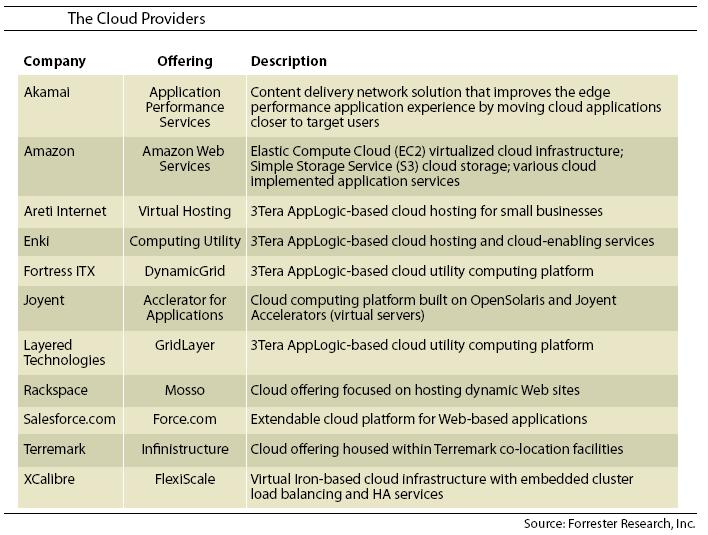
\includegraphics[scale=0.35]{Clould provider.jpg}
\caption{The provider of cloud computing}
\end{figure}
\vspace{.4cm}

Beside that, cost factor is one of the reason for this cloud computing development. In one organisation with quite numbers of employees, the IT administrator had to ensure all the employees have the right software and hardware they need for their jobs. Ideal solution is to purchase computers for everyone with the right software. One thing to remember, each software come with licence requirement. However this solution required huge money and the more employees means the more money they need to invest. Therefore, cloud computing is the correct solution which the only need is to install one application. In this application, each user are allowed to log in to a web-based service which hosts all the programs the user need for his or her jobs. 

\vspace{.5cm}	
\subsection{The Very Best Company for Data Center Management Have the Solution}

The leading Web services companies have built their businesses around innovative new approaches to IT infrastructure that maximize data center management and efficiency � investments that have given them advantage over competitors that came to Web services from a traditional IT foundation. This success led Amazon CTO Werner Vogels to conclude in his keynote address at the 2007 Next Generation Data Center Conference that if managing a massive data center isn�t a core competency of your business.   

Amazon Web Services has since grown into a new business that encompasses compute and storage infrastructure services and new middleware services that Amazon EC2 customers can leverage, such as the Amazon Simple Queue Service. But it isn�t alone. There are host of emerging cloud computing vendors to choose from, some of which are more enterprise-friendly. 

the architectures of the clouds support nearly any type of application the customer may want to host as long as it does not need direct access to the hardware or specialized hardware elements, as shown in Figure 2 the complete architecture of cloud computing .

\begin{figure}
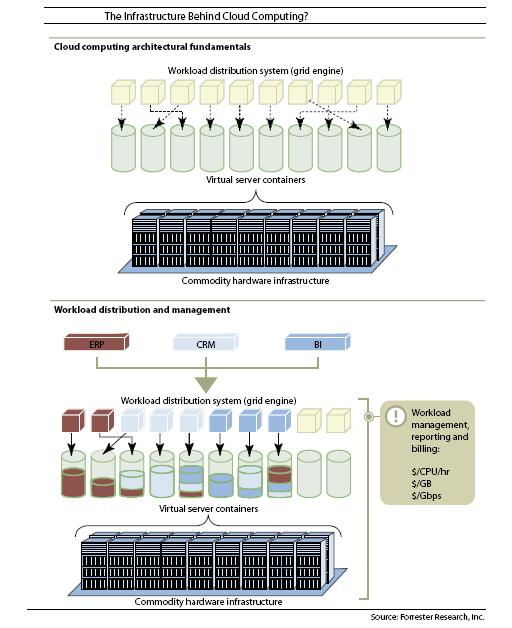
\includegraphics[scale=0.30]{The Cloud Computing Infrastructure.jpg}
\centering
\caption{Cloud Infrastructure}
\end{figure}
\vspace{.4cm}	




\vspace{.5cm}	
\subsection{Web Search Trends}

The popularity of different computing service paradigms varies with time. The Web search popularity, as measured by the Google search trends during the last 12 months, for terms "cluster computing", "Grid computing", and "Cloud computing" is shown in Figure 3. From the Google trends, it can be observed that cluster computing was a popular term during 1990s, from early 2000 Grid computing become popular, and recently Cloud computing started gaining popularity. Spot points in Figure 4 indicate the release of news related to Cloud computing as follows: 

\textbf{
\begin{itemize}
\item     1. IBM Introduces 'Blue Cloud' Computing, CIO Today - Nov 15 2007.
\end{itemize}
}

\textbf{
\begin{itemize}
\item     2. IBM, EU Launch RESERVOIR Research Initiative for Cloud Computing, IT News Online - Feb 7 2008.
\end{itemize}
}

\textbf{
\begin{itemize}
\item     3. Google and Salesforce.com in Cloud computing deal, Siliconrepublic.com - Apr 14 2008. 
\end{itemize}
}

\textbf{
\begin{itemize}
\item     4. Demystifying Cloud Computing, Intelligent Enterprise - Jun 11 2008. 
\end{itemize}
}

\textbf{
\begin{itemize}
\item     5. Yahoo realigns to support Cloud computing, 'core strategies', San Antonio Business Journal - Jun 27 2008. 
\end{itemize}
}

\textbf{
\begin{itemize}
\item     6. Merrill Lynch Estimates "Cloud Computing" To Be 100 Billion Market, SYS-CON Media - Jul 8 2008. 
\end{itemize}
}

\begin{figure}
\center
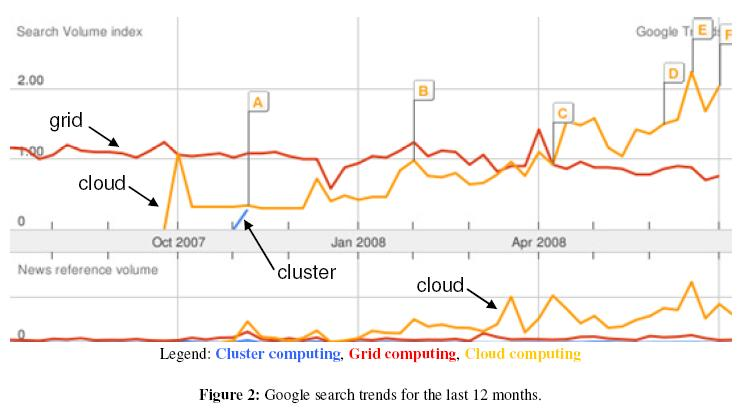
\includegraphics[scale=0.30]{Google search.png}
\caption{Google Search trend for 2008 year}
\end{figure}


\vspace{.3cm}
\section{Emerging Cloud Computing Platforms}

As the computing industry shifts toward providing Platform as a Service (PaaS) and Software as a Service (SaaS) for consumers and enterprises to access on demand regardless of time and location, there will be an increase in the number of Cloud platforms available.

Amazon Elastic Compute Cloud (EC2) [13] provides a virtual computing environment that enables a user to run Linux-based applications. The user can either create a new Amazon Machine Image (AMI) containing the applications, libraries, data and associated configuration settings, or select from a library of globally available AMIs. The user then needs to upload the created or selected AMIs to Amazon Simple Storage Service (S3), before he can start, stop, and monitor instances of the uploaded AMIs. Amazon EC2 charges the user for the time when the instance is alive, while Amazon S3 charges for any data transfer (both upload and download).

Google App Engine [14] allows a user to run Web applications written using the Python programming language. Other than supporting the Python standard  library, Google App Engine also supports Application Programming Interfaces (APIs) for the datastore, Google Accounts, URL fetch, image manipulation, and email services. Google App Engine also provides a Web-based Administration Console for the user to easily manage his running Web applications. Currently, Google App Engine is free to use with up to 500MB of storage and about 5 million page views per month.

Microsoft Live Mesh [15] aims to provide a centralized location for a user to store applications and data that can be accessed across required devices (such as computers and mobile phones) from anywhere in the world. The user is able to access the uploaded applications and data through a Web-based Live Desktop or his own devices with Live Mesh software installed. Each user�s Live Mesh is password-protected and authenticated via his Windows Live Login, while all file transfers are protected using Secure Socket Layers (SSL).

Sun network.com (Sun Grid) [16] enables the user to run Solaris OS, Java, C, C++, and FORTRAN based applications. First, the user has to build and debug his applications and runtime scripts in a local development environment that is configured to be similar to that on the Sun Grid. Then, he needs to create a bundled zip archive (containing all the related scripts, libraries, executable binaries and input data) and upload it to Sun Grid. Finally, he can execute and monitor the application using the Sun Grid Web portal or API.



\begin{figure}
\centering
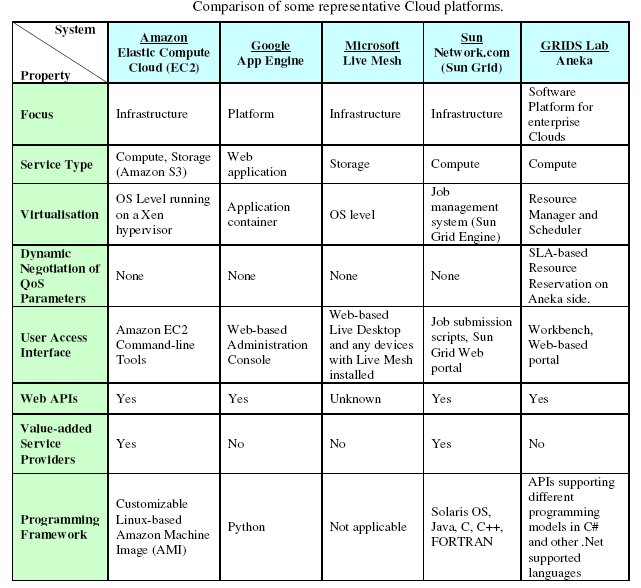
\includegraphics[scale=0.25]{Comparision cloud platform.png}
\caption{Different type of Cloud Computing}
\end{figure}


\subsection{Amazon Web Services: Elastic Compute Cloud}
In 2006 Amazon announced its Simple Storage Service (S3) its Elastic Compute Cloud (EC2). S3 and EC2 together offer a cloud compute and storage resource that provides the possibility of computing on virtual parallel clusters generated and destroyed on demand. EC2 is based on Linux and Xen (3) and various O/S images, Amazon Machine Images (AMIs), can be supported.

%\vspace{.2cm}	

\subsubsection{EC2 Instances}
\vspace{.2cm}	
Currently Amazon EC2 offers five �hardware� instance types with different characteristics (cpu power, memory, disk and addressability) and different pricing. Amazon provides a basic measure of an EC2 Compute Unit (1) for compute power: �One EC2 Compute Unit provides the equivalent CPU capacity of a 1.0-1.2 GHz 2007 Opteron or 2007 Xeon processor.� These instance types have been classified by Amazon as (i) a set of three standard instances called m1.small, m1.large and m1.xlarge (ii) pair of high cpu instances called c1.medium and c1.xlarge. We instantiated all five types and looked at the actual hardware that was provided. It is apparent from the type of cpus encountered that all Amazon EC2 systems we were assigned were dual socket multicore cpus. In the case of the standard instance type, a �half of a core� behavior is enforced by allowing cpu utilization of the single processor virtual machine to be at most 50/100 , a limitation which system utilities such as �top� easily show. For benchmarking one can, therefore, only meaningfully speak of wallclock and not of cpu time on these instances, even in the case of serial codes. Ensuring that no daemons or other processes are contending for cpu time is, therefore, critical for all measurements to be of any use. For cpu intensive applications that spend most of their time with a full pipeline this 50/100 utilization limitation means that one instance is essentially equivalent to a downrated 1.3 GHz Opteron processor (hence the definition of an EC2 Compute Unit). The same cannot necessarily be said for memory bandwidth or memory latency (important quantities for many HPC applications). By virtue of running in a virtual machine environment, we also cannot know at any given moment whether the other cores in our actual physical system (but not in our O/S image) are being used by ourselves or another user. Such co-habitation of the physical system leads to contention for the processor socket bandwidth (for the standard instance type), and the main memory bandwidth (for the medium instance types). The only exceptions to this rule are the xlarge instances that essentially run a single Xen domU virtual machine on top of the base Xen dom0 one for the whole two socket node. The high-cpu instance types employ quad core core processors: while these Core2 architecture based processors are very fast, their effective memory bandwidth is further reduced as 4 processor cores share the same socket pins to the north bridge path to main memory (which is in turn shared with the other socket�s four cores). Within each of the families of instances, pricing is proportional to the number of EC2 Compute Units but compute power wise (based on Amazon�s figure 5) the 32-bit High- CPU instance appears to be more cost-effective. For our work we opted to initially concentrate our tests on the 32-bit images only that are the cheapest to use (at 0.1 and 0.2 per cpu hour respectively).

\begin{figure}
\center
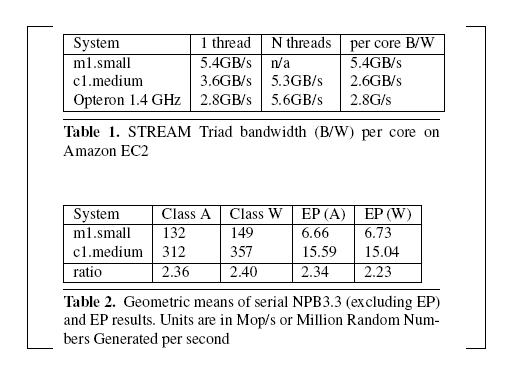
\includegraphics[scale=0.50]{EC2 instances.jpg}
\caption{EC2 instances}
\end{figure}


\vspace{.4cm}	
\section{CLOUD COMPUTING VS GRID COMPUTING}

Of all these computing paradigms, the two most promising ones appear to be Grid computing and Cloud computing.

Cloud computing is not like Grid Computing. Grid Computing is where a group of computers is linked together in a network to performed one very large task. Cloud computing on the other hand, can perform multiple task. It is like a server hosting for multiple application. 

Grid computing has been use in current market where users make a few request which allocate large requirement each. For example, an organization may have 1000  node cluster and group it to few allocation, let say 200.  Unfortunately, only a few allocation can be serve at one time where by the others have to wait and may need to reschedule for other time when the resources are released. This phenomena will results a batch job scheduling algorithms of parallel computations.[1]

Cloud computing is focus to small allocation requests. 
the motivation of Grid computing was initially driven by large-scale, resource (computational and data)-intensive scientific applications that required more resources than a single computer (PC, workstation, supercomputer, or cluster) could have provided in a single administrative domain.
Grid computing has been conceder as the next revolution after the Internet and the Web.
A Grid [3] enables the sharing, selection, and aggregation of a wide variety of geographically distributed resources including supercomputers, storage systems, data sources, and specialized devices owned by different organizations for solving large scale resource-intensive problems in science, engineering, and commerce.
For example Amazon EC2 accounts are limited to 20 servers each and a lot of users allocate up to 20 servers from many thousands of servers someone else release resources. This situation is completely different resource allocation paradigm, usage pattern and results in completely different method of using computer resources. 

Anyway, it not that easy to create a cloud even though it just consist a cloud management software and support by a few computers. On the other hand, it is a challenging to support the apply of real time resource availability. The cloud provider need to provide resources and if they fail, the whole system will collapse and the users will start hoarding servers, resulting a peak usage than normal demand.

Below table shows the summary of comparison between cloud computing and grid computing by using a model from each category.

\section{BENEFITS}

There are many benefits in cloud computing systems. All user either individual or organisation can enjoy many advantages when apply to this new systems. Simple and minimum IT management with low cost requirement makes cloud computing are practically to be use for all kind of user. That is why this new practice is now in rapid development and being popular in IT environment.  

\textbf{
\begin{itemize}
\item Client or users can access their application and data from anywhere at any time. The only needs to be linked to cloud computing system is a computer with internet connection.
\end{itemize}
}

\textbf{
\begin{itemize}
\item It is elastic -- a user can have as much or as little of a service as they want at any given time; and the service is fully managed by the provider (the consumer needs nothing but a personal computer and Internet access); That's meaningful of cloud computing will remove the need for physical space on the front end.
\end{itemize}
}

\textbf{
\begin{itemize}
\item The needs of advance hardware and software are no longer required and could be reduce the hardware and software cost. It means, the user are no longer need to buy the fastest computer with huge memory because the cloud computer system will take care all this requirement. Therefore all the user needs could be a cheaper personal computer with basic and common requirement which can easily get it from the market.
\end{itemize}
}

\textbf{
\begin{itemize}
\item In the cloud computing systems, they can provide this organization an access to their computer application for all the employee. Therefore the need of a set of software with license for all the employee are no longer required. Instead, the company are only required to pay the access fee to the cloud computing company.
\end{itemize}
}

\textbf{
\begin{itemize}
\item The client could have advantages of the entire network's processing power if the cloud computing system's was supported by a grid computing system at the back end. There are many cases that a scientists or researchers works with very complex calculation and take so much time for individual computer to complete them. In this case, cloud computing system will tap into processing power for all available computers in the cloud and resulting reduce the calculation processing time.
\end{itemize}
}

\begin{center}
\section{HOW IT BEING USED}
\end{center}

In global IT environment cloud computing had been used widely besides we may not aware that sometimes we are part of it. Below is some example and how it being used by the user.

\textbf{
\begin{itemize}
\item SaaS
With the development of cloud computing come a new idea of distributing software through Internet. SaaS (Software as a service) is being introduced as a next step of software distribution. Using cloud computing architecture, a single application can be delivered through the browser to the user. On the user side there is no upfront investment in server of software licensing and on the provider side, they only have to maintain one application thus the maintenance cost will greatly reduce. Some examples of SaaS are Saleforce.com, Google Apps and Zoho Office.
\end{itemize}
}

\textbf{
\begin{itemize}
\item Utility computing
This form of cloud computing give a whole new meaning to IT related utility where software is charge just like a public utilities such as electricity or water. Company like Amazon.com, Sun, IBM and other who offer storage and virtual server and customers can access on demand. 
\end{itemize}
}


\section{SECURITY IN CLOUD COMPUTING}

Here are seven of the specific security issues Gartner says customers should raise with vendors before selecting a cloud vendor.

\textbf{
\begin{itemize}
	\item Privileged user access.
\end{itemize}
}
Sensitive data processed outside the enterprise brings with it an inherent level of risk, because outsourced services bypass the "physical, logical and personnel controls" IT shops exert over in-house programs. Get as much information as you can about the people who manage your data. "Ask providers to supply specific information on the hiring and oversight of privileged administrators, and the controls over their access," Gartner says.

\textbf{
\begin{itemize}
	\item Regulatory compliance 
\end{itemize}
}
Customers are ultimately responsible for the security and integrity of their own data, even when it is held by a service provider. Traditional service providers are subjected to external audits and security certifications. Cloud computing providers who refuse to undergo this scrutiny are "signaling that customers can only use them for the most trivial functions," according to Gartner. 

\textbf{
\begin{itemize}
	\item Data location. 
\end{itemize}
}
When you use the cloud, you probably won't know exactly where your data is hosted. In fact, you might not even know what country it will be stored in. Ask providers if they will commit to storing and processing data in specific jurisdictions, and whether they will make a contractual commitment to obey local privacy requirements on behalf of their customers, Gartner advises.

\textbf{
\begin{itemize}
	\item Data segregation.
\end{itemize}
} 
Data in the cloud is typically in a shared environment alongside data from other customers. Encryption is effective but isn't a cure-all. "Find out what is done to segregate data at rest," Gartner advises. The cloud provider should provide evidence that encryption schemes were designed and tested by experienced specialists. "Encryption accidents can make data totally unusable, and even normal encryption can complicate availability," Gartner says.

\textbf{
\begin{itemize}
	\item Recovery. 
\end{itemize}
}
Even if you don't know where your data is, a cloud provider should tell you what will happen to your data and service in case of a disaster. "Any offering that does not replicate the data and application infrastructure across multiple sites is vulnerable to a total failure," Gartner says. Ask your provider if it has "the ability to do a complete restoration, and how long it will take."

\textbf{
\begin{itemize}
	\item Investigative support. 
\end{itemize}
}
Investigating inappropriate or illegal activity may be impossible in cloud computing, Gartner warns. "Cloud services are especially difficult to investigate, because logging and data for multiple customers may be co-located and may also be spread across an ever-changing set of hosts and data centers. If you cannot get a contractual commitment to support specific forms of investigation, along with evidence that the vendor has already successfully supported such activities, then your only safe assumption is that investigation and discovery requests will be impossible."

\textbf{
\begin{itemize}
	\item Long-term viability.
\end{itemize}
}
Ideally, your cloud computing provider will never go broke or get acquired and swallowed up by a larger company. But you must be sure your data will remain available even after such an event. "Ask potential providers how you would get your data back and if it would be in a format that you could import into a replacement application," Gartner says.


\section{CLOUD COMPUTING FOR MALAYSIAN GOVERMENT}
Cloud computing is still in its early stages, but the public sector is already beginning to see advantages. Despite its possible security and privacy risks, Cloud Computing  according to a magazine article due to be published later this Fall  has six main benefits that the public sector and government IT organizations are certain to want to take advantage of. In very brief summary form they are as follows:

\textbf{
\begin{itemize}
	\item Reduced Cost
\end{itemize}
}
Cloud technology is paid incrementally, saving organizations money. 

\textbf{
\begin{itemize}
	\item Increased Storage
\end{itemize}
}
Organizations can store more data than on private computer systems. 

\textbf{
\begin{itemize}
	\item Highly Automated 
\end{itemize}
}
No longer do IT personnel need to worry about keeping software up to date. 

\textbf{
\begin{itemize}
	\item Flexibility
\end{itemize}
}
Cloud computing offers much more flexibility than past computing methods. 

\textbf{
\begin{itemize}
	\item More Mobility 
\end{itemize}
}
Employees can access information wherever they are, rather than having to remain at their desks. 

\textbf{
\begin{itemize}
	\item Allows IT to Shift Focus
\end{itemize}
}
No longer having to worry about constant server updates and other computing issues, government organizations will be free to concentrate on innovation. 


% You must have at least 2 lines in the paragraph with the drop letter
% (should never be an issue)

%\hfill 
 
%\hfill September 1, 2009

% An example of a floating figure using the graphicx package.
% Note that \label must occur AFTER (or within) \caption.
% For figures, \caption should occur after the \includegraphics.
% Note that IEEEtran v1.7 and later has special internal code that
% is designed to preserve the operation of \label within \caption
% even when the captionsoff option is in effect. However, because
% of issues like this, it may be the safest practice to put all your
% \label just after \caption rather than within \caption{}.
%
% Reminder: the "draftcls" or "draftclsnofoot", not "draft", class
% option should be used if it is desired that the figures are to be
% displayed while in draft mode.
%
%\begin{figure}[!t]
%\centering
%\includegraphics[width=2.5in]{myfigure}
% where an .eps filename suffix will be assumed under latex, 
% and a .pdf suffix will be assumed for pdflatex; or what has been declared
% via \DeclareGraphicsExtensions.
%\caption{Simulation Results}
%\label{fig_sim}
%\end{figure}

% Note that IEEE typically puts floats only at the top, even when this
% results in a large percentage of a column being occupied by floats.


% An example of a double column floating figure using two subfigures.
% (The subfig.sty package must be loaded for this to work.)
% The subfigure \label commands are set within each subfloat command, the
% \label for the overall figure must come after \caption.
% \hfil must be used as a separator to get equal spacing.
% The subfigure.sty package works much the same way, except \subfigure is
% used instead of \subfloat.
%
%\begin{figure*}[!t]
%\centerline{\subfloat[Case I]\includegraphics[width=2.5in]{subfigcase1}%
%\label{fig_first_case}}
%\hfil
%\subfloat[Case II]{\includegraphics[width=2.5in]{subfigcase2}%
%\label{fig_second_case}}}
%\caption{Simulation results}
%\label{fig_sim}
%\end{figure*}
%
% Note that often IEEE papers with subfigures do not employ subfigure
% captions (using the optional argument to \subfloat), but instead will
% reference/describe all of them (a), (b), etc., within the main caption.


% An example of a floating table. Note that, for IEEE style tables, the 
% \caption command should come BEFORE the table. Table text will default to
% \footnotesize as IEEE normally uses this smaller font for tables.
% The \label must come after \caption as always.
%
%\begin{table}[!t]
%% increase table row spacing, adjust to taste
%\renewcommand{\arraystretch}{1.3}
% if using array.sty, it might be a good idea to tweak the value of
% \extrarowheight as needed to properly center the text within the cells
%\caption{An Example of a Table}
%\label{table_example}
%\centering
%% Some packages, such as MDW tools, offer better commands for making tables
%% than the plain LaTeX2e tabular which is used here.
%\begin{tabular}{|c||c|}
%\hline
%One & Two\\
%\hline
%Three & Four\\
%\hline
%\end{tabular}
%\end{table}


% Note that IEEE does not put floats in the very first column - or typically
% anywhere on the first page for that matter. Also, in-text middle ("here")
% positioning is not used. Most IEEE journals/conferences use top floats
% exclusively. Note that, LaTeX2e, unlike IEEE journals/conferences, places
% footnotes above bottom floats. This can be corrected via the \fnbelowfloat
% command of the stfloats package.



% conference papers do not normally have an appendix


% use section* for acknowledgement
\section{Summary and Conclusion}
Cloud computing is a new and promising paradigm delivering IT services as computing utilities. 
As Clouds are designed to provide services to external users, providers need to be compensated for sharing their resources and capabilities. 

From the current situation, cloud computing technologies are still immature, which may lead to problems in service management and usability. 
However  the potential of cloud computing benefit will make it interesting and therefore many people will participate in the progress and development of it. 
There will be more challenges on this technology, but it will not make it stop. 
Furthermore it will growth just like the internet today and will be commonly use in the near future.


\section*{Acknowledgment}
The Researcher Mohammed Altemimi would like to thank Dr. Mohd Zamri to give us these very valuable information ...

% trigger a \newpage just before the given reference
% number - used to balance the columns on the last page
% adjust value as needed - may need to be readjusted if
% the document is modified later
%\IEEEtriggeratref{8}
% The "triggered" command can be changed if desired:
%\IEEEtriggercmd{\enlargethispage{-5in}}

% references section

% can use a bibliography generated by BibTeX as a .bbl file
% BibTeX documentation can be easily obtained at:
% http://www.ctan.org/tex-archive/biblio/bibtex/contrib/doc/
% The IEEEtran BibTeX style support page is at:
% http://www.michaelshell.org/tex/ieeetran/bibtex/
%\bibliographystyle{IEEEtran}
% argument is your BibTeX string definitions and bibliography database(s)
%\bibliography{IEEEabrv,../bib/paper}
%
% <OR> manually copy in the resultant .bbl file
% set second argument of \begin to the number of references
% (used to reserve space for the reference number labels box)






\begin{thebibliography}{1}


\bibitem{IEEEhowto:kopka}
L. Kleinrock , \emph{Avision for the Internet}, \hskip , \emph \ST Journal of research, 2(1):4-4,Nov. 2005.

\bibitem{IEEEhowto:kopka}
Morgan Stanley. Technology Trends. 12 June 2008 \emph{ } \emph  \hskip \relax http://www.monganstanley.com/institutional/techresearch/pdfs/TecchTrends062008.pdf [18 July 2008]

\bibitem{IEEEhowto:kopka}
1.Foster and C.Kesselman (eds) , \emph{The Grid: Blue Print for a future Computing Infrastructure}, \hskip , \emph \Morgan Kaufmann, San Francisco, USA ,1999.

\bibitem{IEEEhowto:kopka}
I. Liorente, OpenNebuala Project. \emph{ } \emph, \relax http://www.opennebula.org [238 July 2008].

\bibitem{IEEEhowto:kopka}
A.Weiss., \emph{Computing in the Clouds}, \hskip , \emph, \netWorkers 11(4):16-25, Dos- 2007.

\bibitem{IEEEhowto:kopka}
Nurmi, Rich Wolski, Chris Grzegorczyk Graziano Obertelli, Sunil Soman, Lamia Youseff, Dmitrii Zagorodnov, \emph{The Eucalyptus Open-source Cloud- computing System }, \hskip  \emph \relax ACM pp.1�5.


\bibitem{IEEEhowto:kopka}
Amazon elastic compute cloud, \emph{} \emph \relax http://aws.amazon.com/ec2

\bibitem{IEEEhowto:kopka}
Enomalism elastic computing infrastructure, \emph{} \emph \relax http:// www.enomaly.com


\bibitem{IEEEhowto:kopka}
K. Keahey, I. Foster, T. Freeman, and X. Zhang, \emph{Virtual workspaces: Achieving quality of service and quality of life in the grid}, \hskip \emph \relax Sci. Program., 13(4):265�275, 2005.

\bibitem{IEEEhowto:kopka}
J. Chase, D. Irwin, L. Grit, J. Moore, and S. Sprenkle, \emph{Dynamic virtual clusters in a grid site manager}, \hskip \emph \relax High Performance Distributed Computing, 2003. Proceedings. 2th IEEE International Symposium on, pages 90�100, 2003.

\bibitem{IEEEhowto:kopka}
M. McNett, D. Gupta, A. Vahdat, and G. M. Voelker, \emph{Usher: An Extensible Framework for Managing Clusters of Virtual Machines}, \hskip , \emph, \relax In Proceedings of the 21st Large Installation System Administration Conference (LISA), November 2007.

\bibitem{IEEEhowto:kopka}
Twenty Experts Define Cloud Computing , \emph{} \emph \relax http://cloudcomputing.sys-con.com/read/612375_p.htm[18 July 2008].

\bibitem{IEEEhowto:kopka}
Amazon Elastic Compute Cloud (EC2), \emph{} \emph \relax http://www.azazon.com/ec2/[18 July 2008].

\bibitem{IEEEhowto:kopka}
Google App Engine, \emph{} \emph \relax http://appengine.google.com [18 July 2008].

\bibitem{IEEEhowto:kopka}
Microsoft Live Mesh, \emph{} \emph \relax http://www.mesh.com [18 July 2008].

\bibitem{IEEEhowto:kopka}
Sunnetwork.com (Sun Grid), \emph{} \emph \relax http://www.network.com [18 July 2008].


\end{thebibliography}

% that's all folks
\end{document}



